\section{Результаты}
	Описанные подходы были реализованы в виде компьютерных программ на языке Python с помощью библиотеки для построения искусственных нейронных сетей Keras \cite{keras}, которая, в свою очередь, использует для расчетов библиотеку Tensorflow \cite{tf}. Использованные версии программных пакетов указаны в Приложении 1. Обучение проводилось на синтетических данных, сгенерированных самостоятельно реализованным генератором. 
	\subsection{Выборки с реализацией одного тренда}
		\subsubsection{Выборка 1}
			% sand:trend 2
			Выборка состояла из 3000 обучающих изображений и 500 валидационных. Все изображения содержали в себе различные случайные реализации одного тренда интенсивности
			$$тут формула \lambda(x) = 0.2 + 0.01875x : \lambda_i = 0.2, \quad \lambda_f = 5$$
			Примеры синтеза, полученные с помощью нейросетей с различными параметрами, приведены в (Таб. \ref{8-dataset1-images}).
			\begin{table}[h]
				\begin{center}
					\begin{tabular}{p{2cm} p{2cm} p{2cm} p{2cm} p{2cm} p{2cm} p{2cm}}
						\toprule
						Вход 1 & Вход 2 & Тренд & Сеть nf8 & nf16 & nf16woU & nf32 \\
						\cmidrule(r){1-1}\cmidrule(lr){2-2}\cmidrule(lr){3-3}\cmidrule(lr){4-4}\cmidrule(lr){5-5}\cmidrule(lr){6-6}\cmidrule(l){7-7}
						
\includegraphics[width=1\linewidth]{8-results/sand-trend2/left1}
						&
						
\includegraphics[width=1\linewidth]{8-results/sand-trend2/right1}
						&
						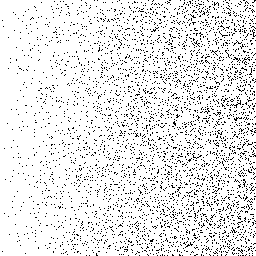
\includegraphics[width=1\linewidth]{8-results/sand-trend2/pan1}
						&
						
\includegraphics[width=1\linewidth]{8-results/sand-trend2/nf8/gen1}
						&
						
\includegraphics[width=1\linewidth]{8-results/sand-trend2/nf16/gen1}
						&
						
\includegraphics[width=1\linewidth]{8-results/sand-trend2/nf16_woUnet/gen1}
						&
						
\includegraphics[width=1\linewidth]{8-results/sand-trend2/nf32/gen1}
						\\
						
\includegraphics[width=1\linewidth]{8-results/sand-trend2/left2}
						&
						
\includegraphics[width=1\linewidth]{8-results/sand-trend2/right2}
						&
						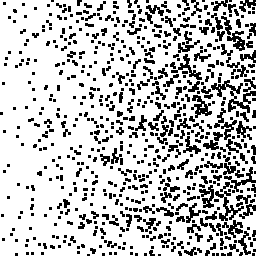
\includegraphics[width=1\linewidth]{8-results/sand-trend2/pan2}
						&
						\includegraphics[width=1\linewidth]{8-results/sand-trend2/nf8/gen2}
						&
						\includegraphics[width=1\linewidth]{8-results/sand-trend2/nf16/gen2}
						&
						\includegraphics[width=1\linewidth]{8-results/sand-trend2/nf16_woUnet/gen2}
						&
						\includegraphics[width=1\linewidth]{8-results/sand-trend2/nf32/gen2}
						\\
						
\includegraphics[width=1\linewidth]{8-results/sand-trend2/left3}
						&
						
\includegraphics[width=1\linewidth]{8-results/sand-trend2/right3}
						&
						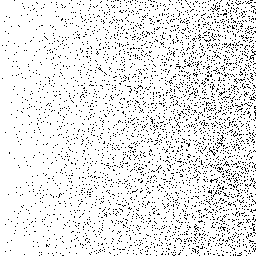
\includegraphics[width=1\linewidth]{8-results/sand-trend2/pan3}
						&
						\includegraphics[width=1\linewidth]{8-results/sand-trend2/nf8/gen3}
						&
						\includegraphics[width=1\linewidth]{8-results/sand-trend2/nf16/gen3}
						&
						\includegraphics[width=1\linewidth]{8-results/sand-trend2/nf16_woUnet/gen3}
						&
						\includegraphics[width=1\linewidth]{8-results/sand-trend2/nf32/gen3}
						\\
						
\includegraphics[width=1\linewidth]{8-results/sand-trend2/left4}
						&
						
\includegraphics[width=1\linewidth]{8-results/sand-trend2/right4}
						&
						
\includegraphics[width=1\linewidth]{8-results/sand-trend2/pan4}
						&
						\includegraphics[width=1\linewidth]{8-results/sand-trend2/nf8/gen4}
						&
						\includegraphics[width=1\linewidth]{8-results/sand-trend2/nf16/gen4}
						&
						\includegraphics[width=1\linewidth]{8-results/sand-trend2/nf16_woUnet/gen4}
						&
						\includegraphics[width=1\linewidth]{8-results/sand-trend2/nf32/gen4}
						\\
						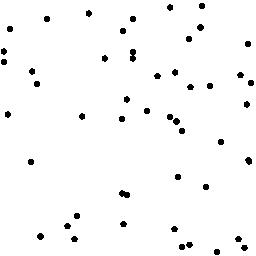
\includegraphics[width=1\linewidth]{8-results/sand-trend2/left5}
						&
						
\includegraphics[width=1\linewidth]{8-results/sand-trend2/right5}
						&
						
\includegraphics[width=1\linewidth]{8-results/sand-trend2/pan5}
						&
						
\includegraphics[width=1\linewidth]{8-results/sand-trend2/nf8/gen5}
						&
						
\includegraphics[width=1\linewidth]{8-results/sand-trend2/nf16/gen5}
						&
						
\includegraphics[width=1\linewidth]{8-results/sand-trend2/nf16_woUnet/gen5}
						&
						
\includegraphics[width=1\linewidth]{8-results/sand-trend2/nf32/gen5}
						\\
						\hline
					\end{tabular}
					\caption{Примеры синтеза (Выборка 1)}
					\label{8-dataset1-images}
				\end{center}
			\end{table}
			\\тут метрики, графики
		\subsubsection{Выборка 2}
			% sand:trend 8
			Выборка состояла из 6000 обучающих изображений и 316 валидационных. Все изображения содержали в себе различные случайные реализации одного тренда интенсивности
			$$тут формула \lambda(x) = 1 + 0.0546875x: \lambda_i = 1, \quad \lambda_f = 15$$
			тут картинки примеров из обучающей выборки \\
			тут сгенерированные семплы \\
			тут метрики, графики
		\subsubsection{Выборка 3}
			% dust:trend 1
			Выборка состояла из 6000 обучающих изображений и 316 валидационных. Все изображения содержали в себе различные случайные реализации одного тренда интенсивности
			$$тут формула \lambda(x) = 1 + 0.19140625x: \lambda_i = 1, \quad \lambda_f = 50$$
			тут картинки примеров из обучающей выборки \\
			тут сгенерированные семплы \\
			тут метрики, графики
		
	\subsection{Выборки с реализацией различных трендов}
		\subsubsection{Выборка 4}
			% dust: trend 2
			Выборка состояла из 6000 обучающих изображений и 316 валидационных. Все изображения содержали в себе различные случайные реализации различных случайных трендов интенсивности $\lambda(x)$ \\
			тут картинки примеров из обучающей выборки \\
			тут сгенерированные семплы \\
			тут метрики, графики